% !TEX root = /Users/zhuzhuangdi/Desktop/MSUCourses/MachineLearning847/17spr_wang_zhu_du/Final/final_report.tex
\section{Methods}
To automatically generate Song Ci, first, we pre-process the Song Ci corpus by mapping each character to a vector representation using a word-embedding matrix, which was previously trained using all corpus in our dataset. 
%
Then we use each character's vector representation as input to train our GA model, RNN model, and GAN model, respectively.
%Then we use a vector space model to convert each Chinese character in the corpus to be a vector presentation in the vector space so that characters with similar semantic meanings have small distance in the vector space.
%
%Using the vector space as training data, we build a Recurrent Neural Network (RNN) that can generate Song Ci with coherent and poetic meanings.
%We add Long short-term memory (LSTM) units in our RNN model to capture long-term semantic dependencies in Song Ci.

\subsection{Preprocessing}
We use word embedding to map Chinese characters from the poem corpus to vectors of real numbers, which consists of two steps: tokenization and word embedding.
% 
%Especially, we consider both semantic and rhythmic relevance in the word-to-vector transformation.
%
\subsubsection {Tokenization}
%
We associated each Chinese character with a unique value as its ID, so that the most frequent word in the corpus  will get a highest value, while the less frequent words have smaller ones.
%
During our project, we carefully tune the size of the vocabulary set $|V|$ so that the most $|V|$ frequent words will be kept in our vocabulary, while the other unfrequent words will be mapped to the same \emph{UNKOWN} token to avoid overfitting.
%
Then we use the ID as the feature for each word to train our word embedding matrix.
%Each character has a unique index ID, while characters share the same simple or compound vowels will have the same rhyme ID. 
%For example, in Figure \ref{fig:rhyme_features}, the two Chinese characters, \emph{guang} and \emph{shuang}, will maintain the same rhyme ID.
%The rhymes can be extracted using a python module called \emph{pinyin}.
%
%
%\begin{figure}[htb]
%	\centering
%	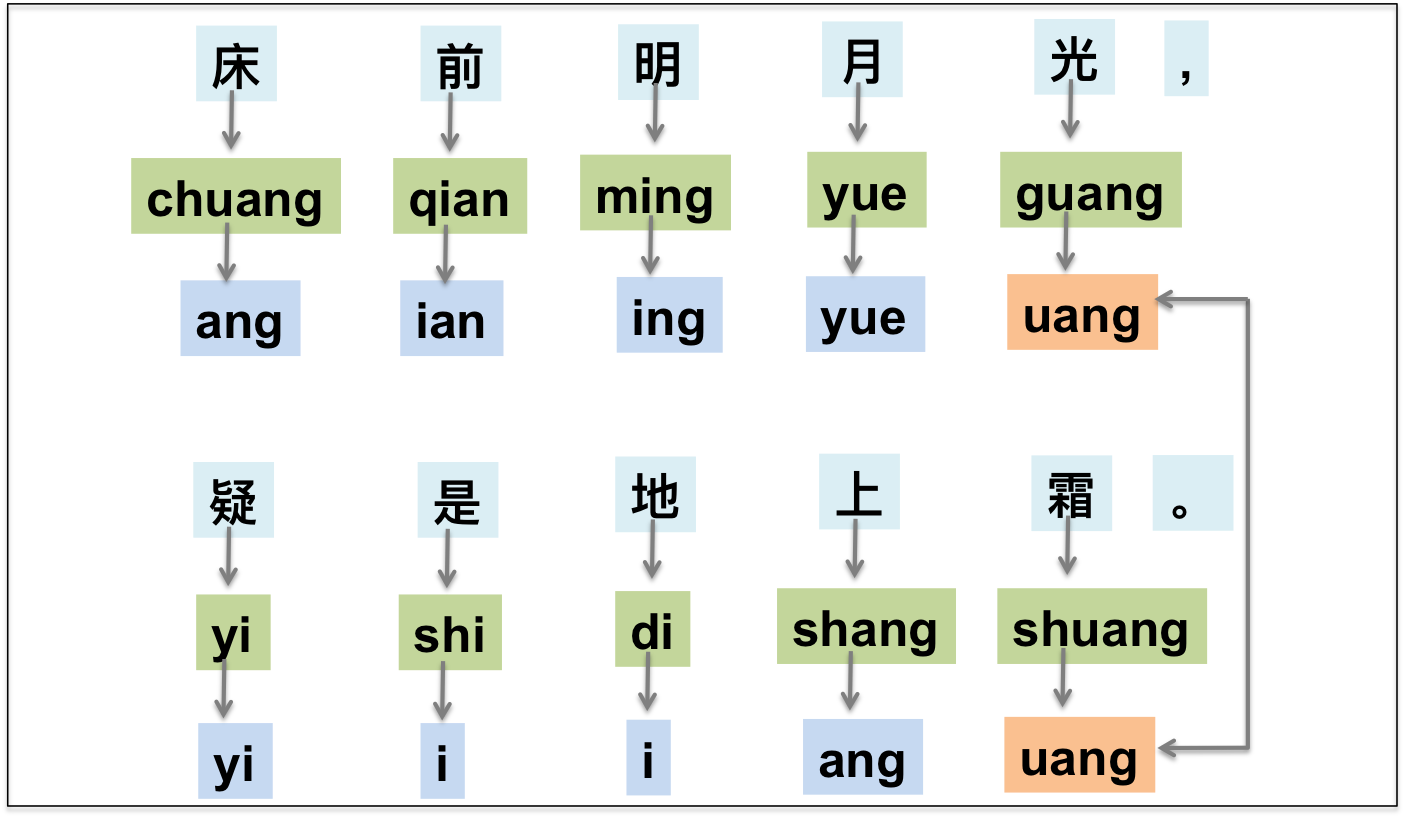
\includegraphics[width=0.9\linewidth]{rhyme_input}
%	\caption{Extracting rhythmic features}
%	\label{fig:rhyme_features}
%\end{figure}

\subsubsection {Word Embedding Using Skip-Gram Model}
We will create a word embedding matrix by training the skip-gram mode which is a single-layer neural network. 
%and the parameter matrix inside the network will be our word embedding matrix.
%
 The input of the model is a single word $w_I$, and the output is the words in its context $\{w_{O,1},w_{O,2}, \dots, w_{O,C}\}$ defined by a word window of size $C$.
%
As shown in Figure \ref{fig:skip_gram},  $x$ represents the one-hot encoded vector corresponding to the
input word in the training text,
%
 and $\{y_1, y_2, \dots, y_C\}$ are the one-hot encoded vectors corresponding to the output words in the training text.
 %
 The $V \times N$ matrix $W$ is the weight matrix between the input layer and hidden layer whose
$i^{th}$ row represents the weights corresponding to the $i^{th}$ word in the vocabulary. 
%
This weight matrix is what we call the word-embedding matrix because it contains the
vector encodings of all of the words in our vocabulary.

\begin{figure}[htb]
	\centering
	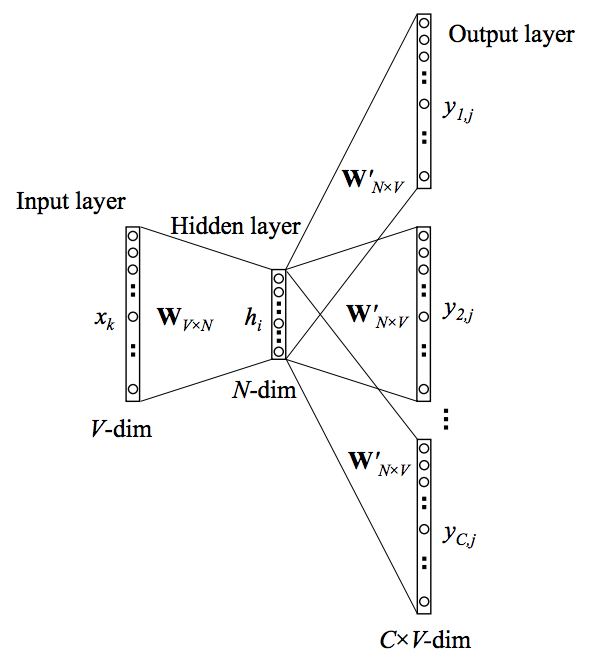
\includegraphics[width=0.9\linewidth]{skip_gram}
	\caption{A skip gram neural network}
	\label{fig:skip_gram}
\end{figure} 
 
\subsection{Genetic Algorithm}
Genetic algorithm(GA) belongs to the class of evolutionary algorithms(EA).
%
It is inspired by the process of natural evolution. Operations in biological evolution process such as mutation, crossover and selection are used in genetic algorithm\cite{banzhaf1998genetic}.
%
Genetic algorithm employ operations close to random search for locating the globally optimal solutions.
%
Since the first time genetic algorithm was proposed by Holland\cite{holland1975adaptation} in 1975, it has been studied and developed for nearly 40 years.
%
It is widely used in many areas, especially for optimization and search problems.


In genetic algorithm, the initial population which is a group of candidate solutions are randomly generated based on the nature of the problem.
%
Each individual has a set of properties which can be mutated and altered.
%
Evolution is a following iterative process, population in each iteration is called a generation.
%
In each generation, the fitness value of each individual is evaluated.
%
Fitness value is calculated by the objective function in the optimization problem that is used to evaluate the performance of the solutions.
%
The most fit individuals are selected under some strategy to become parents. The properties of those selected individuals will be modified to form new individuals.
%
Modification of individuals include recombination and possibly randomly mutation.
%
The new generation will enter the next iteration of the algorithm.
%
When the population reached a certain stop criteria, for example a satisfactory fitness level has been reached or a maximum number of generations has been produced.
 
\subsection{Recurrent Neural Network}  
RNNs are the family of the deep learning structures to process sequential data  \cite{rumelhart1986}.
%
It is specialized for processing a sequence of valuesx $x^{(1)}, x^{(2)}, \dots, x^{(t)}$.
%
Parameter sharing across the different parts of the model is the key idea that makes RNNs to be able to deal with the sequential data.
%
However, a simple RNNs cannot learn long time dependency as in the optimization this term tends to vanish or explode very fast \cite{goodfellow2016deeplearning}.
%
To solve this challenge, gated RNNs is proposed and becomes one of the most effective practical models that used for sequential data.
\begin{figure}[htbp]
	\centering
	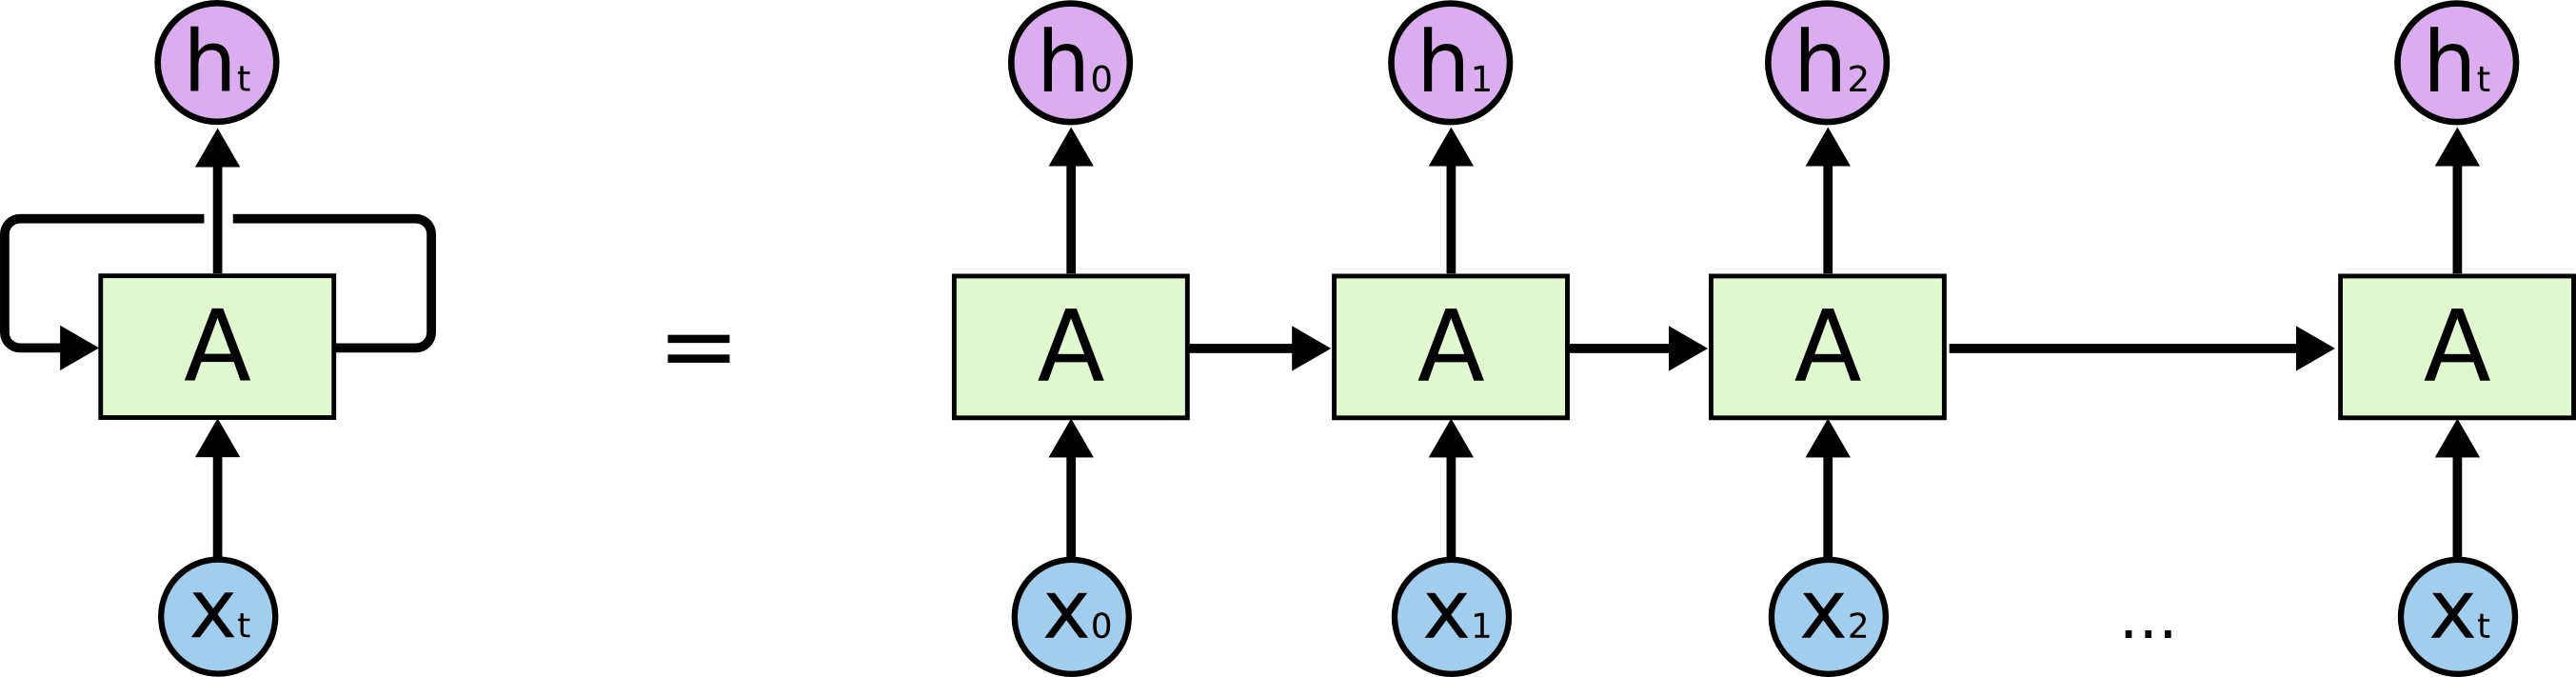
\includegraphics[width=0.9\linewidth]{rnn_overview}
	\caption{A Recurrent Neural Network}
	\label{fig:rnn_overview}
\end{figure}

\subsubsection{Long Short Term Memory}
Long short-term memory (LSTM) model \cite{hochreiter1997lstm} is one branch of such gated RNNs that is extremely successful in the application like speech recognition, machine translation, and handwriting generation.
%
The key idea of LSTM is to introduce a self loop so that gradient can flow for long duration. As shown in Figure \ref{fig:lstm}, the self loop (internal recurrence) is located in "LSTM cells" with outer recurrence like ordinary recurrent network. The weight of self-loop is controlled by a forget gate \(f_i^{(t)}\)
:
\[f_i^{(t)} = \sigma (b_i^f + \sum_{j}U_{i,j}^f x_j^{(t)} +\sum_{j}W_{i,j}^f h_j^{(t-1)} ) \]
Where \(\boldsymbol{x}^{(t)}\) is the current input vector and \(\boldsymbol{h}^{(t)}\) is the current hidden layer vector, containing the outputs of all the LSTM cells. \(\boldsymbol{b}^f\), \(\boldsymbol{U}^f\), and \(\boldsymbol{W}^f\) are biases, input weights, and recurrent weights of the forget gate, respectively. The internal state of LSTM cell is updated with the following equation:
\begin{small}
\[s_i^{(t)} = f_i^{(t)}s_i^{(t-1)}+g_i^{(t)}\sigma(b_i + \sum_{j}U_{i,j}^f x_j^{(t)} +\sum_{j}W_{i,j}^f h_j^{(t-1)} )\]
\end{small}
And the external input gate unit
\(g_i^{(t)} \)
is computed with the following equation:
\[g_i^{(t)} = \sigma (b_i^g + \sum_{j}U_{i,j}^g x_j^{(t)} +\sum_{j}W_{i,j}^g h_j^{(t-1)} ) \]
The output
\(h^{(t)}\)
and the output gate
\(q_i^{(t)}\)
, are updated using sigmoid function also:
\begin{eqnarray*}
h_i^{(t)} &=& \tanh (s_i^{(t)})q_i^{(t)}\\
q_i^{(t)} &=& \sigma (b_i^o + \sum_{j}U_{i,j}^o x_j^{(t)} +\sum_{j}W_{i,j}^o h_j^{(t-1)} )
\end{eqnarray*}

LSTM is proven to be able to learn long-term dependencies more effectively than normal RNNs. In our project, we will use LSTM as our main method. We also plan to compare LSTM performance with other network structures.
\begin{figure}[htb]
	\centering
	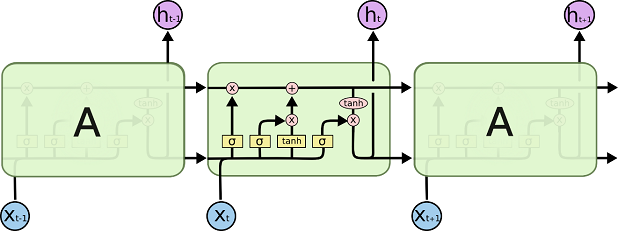
\includegraphics[width=0.9\linewidth]{lstm}
	\caption{A Long Short Term Memory network}
	\label{fig:lstm}
\end{figure} 

\subsection{Generative Adversarial Networks}
Deep generative model is one of the most promising approached to achieve the target than analyze and understand real-word data, such like image, video, and text. The main characteristic of generative model is trying to model the distribution of input implicitly or explicitly \cite{christopher2006prml}. So it possible to generate synthetic data points in the input space.

Differentiable generator network is the key idea for many different generative models. Neural network can be treated as a differentiable function $ g(\bm{z};\bm{\theta}^{(g)}) $, transforming sample of latent variables $ \mathbf{z} $ to samples $ \mathbf{x} $ or to distributions over $ \mathbf{x} $ \cite{goodfellow2016deeplearning}.

Generative Adversarial Network (GANs) \cite{goodfellow2014gan} is a very popular different generative models by pairing the generator network with a discriminator network.

\begin{figure}[htbp]
	\centering
	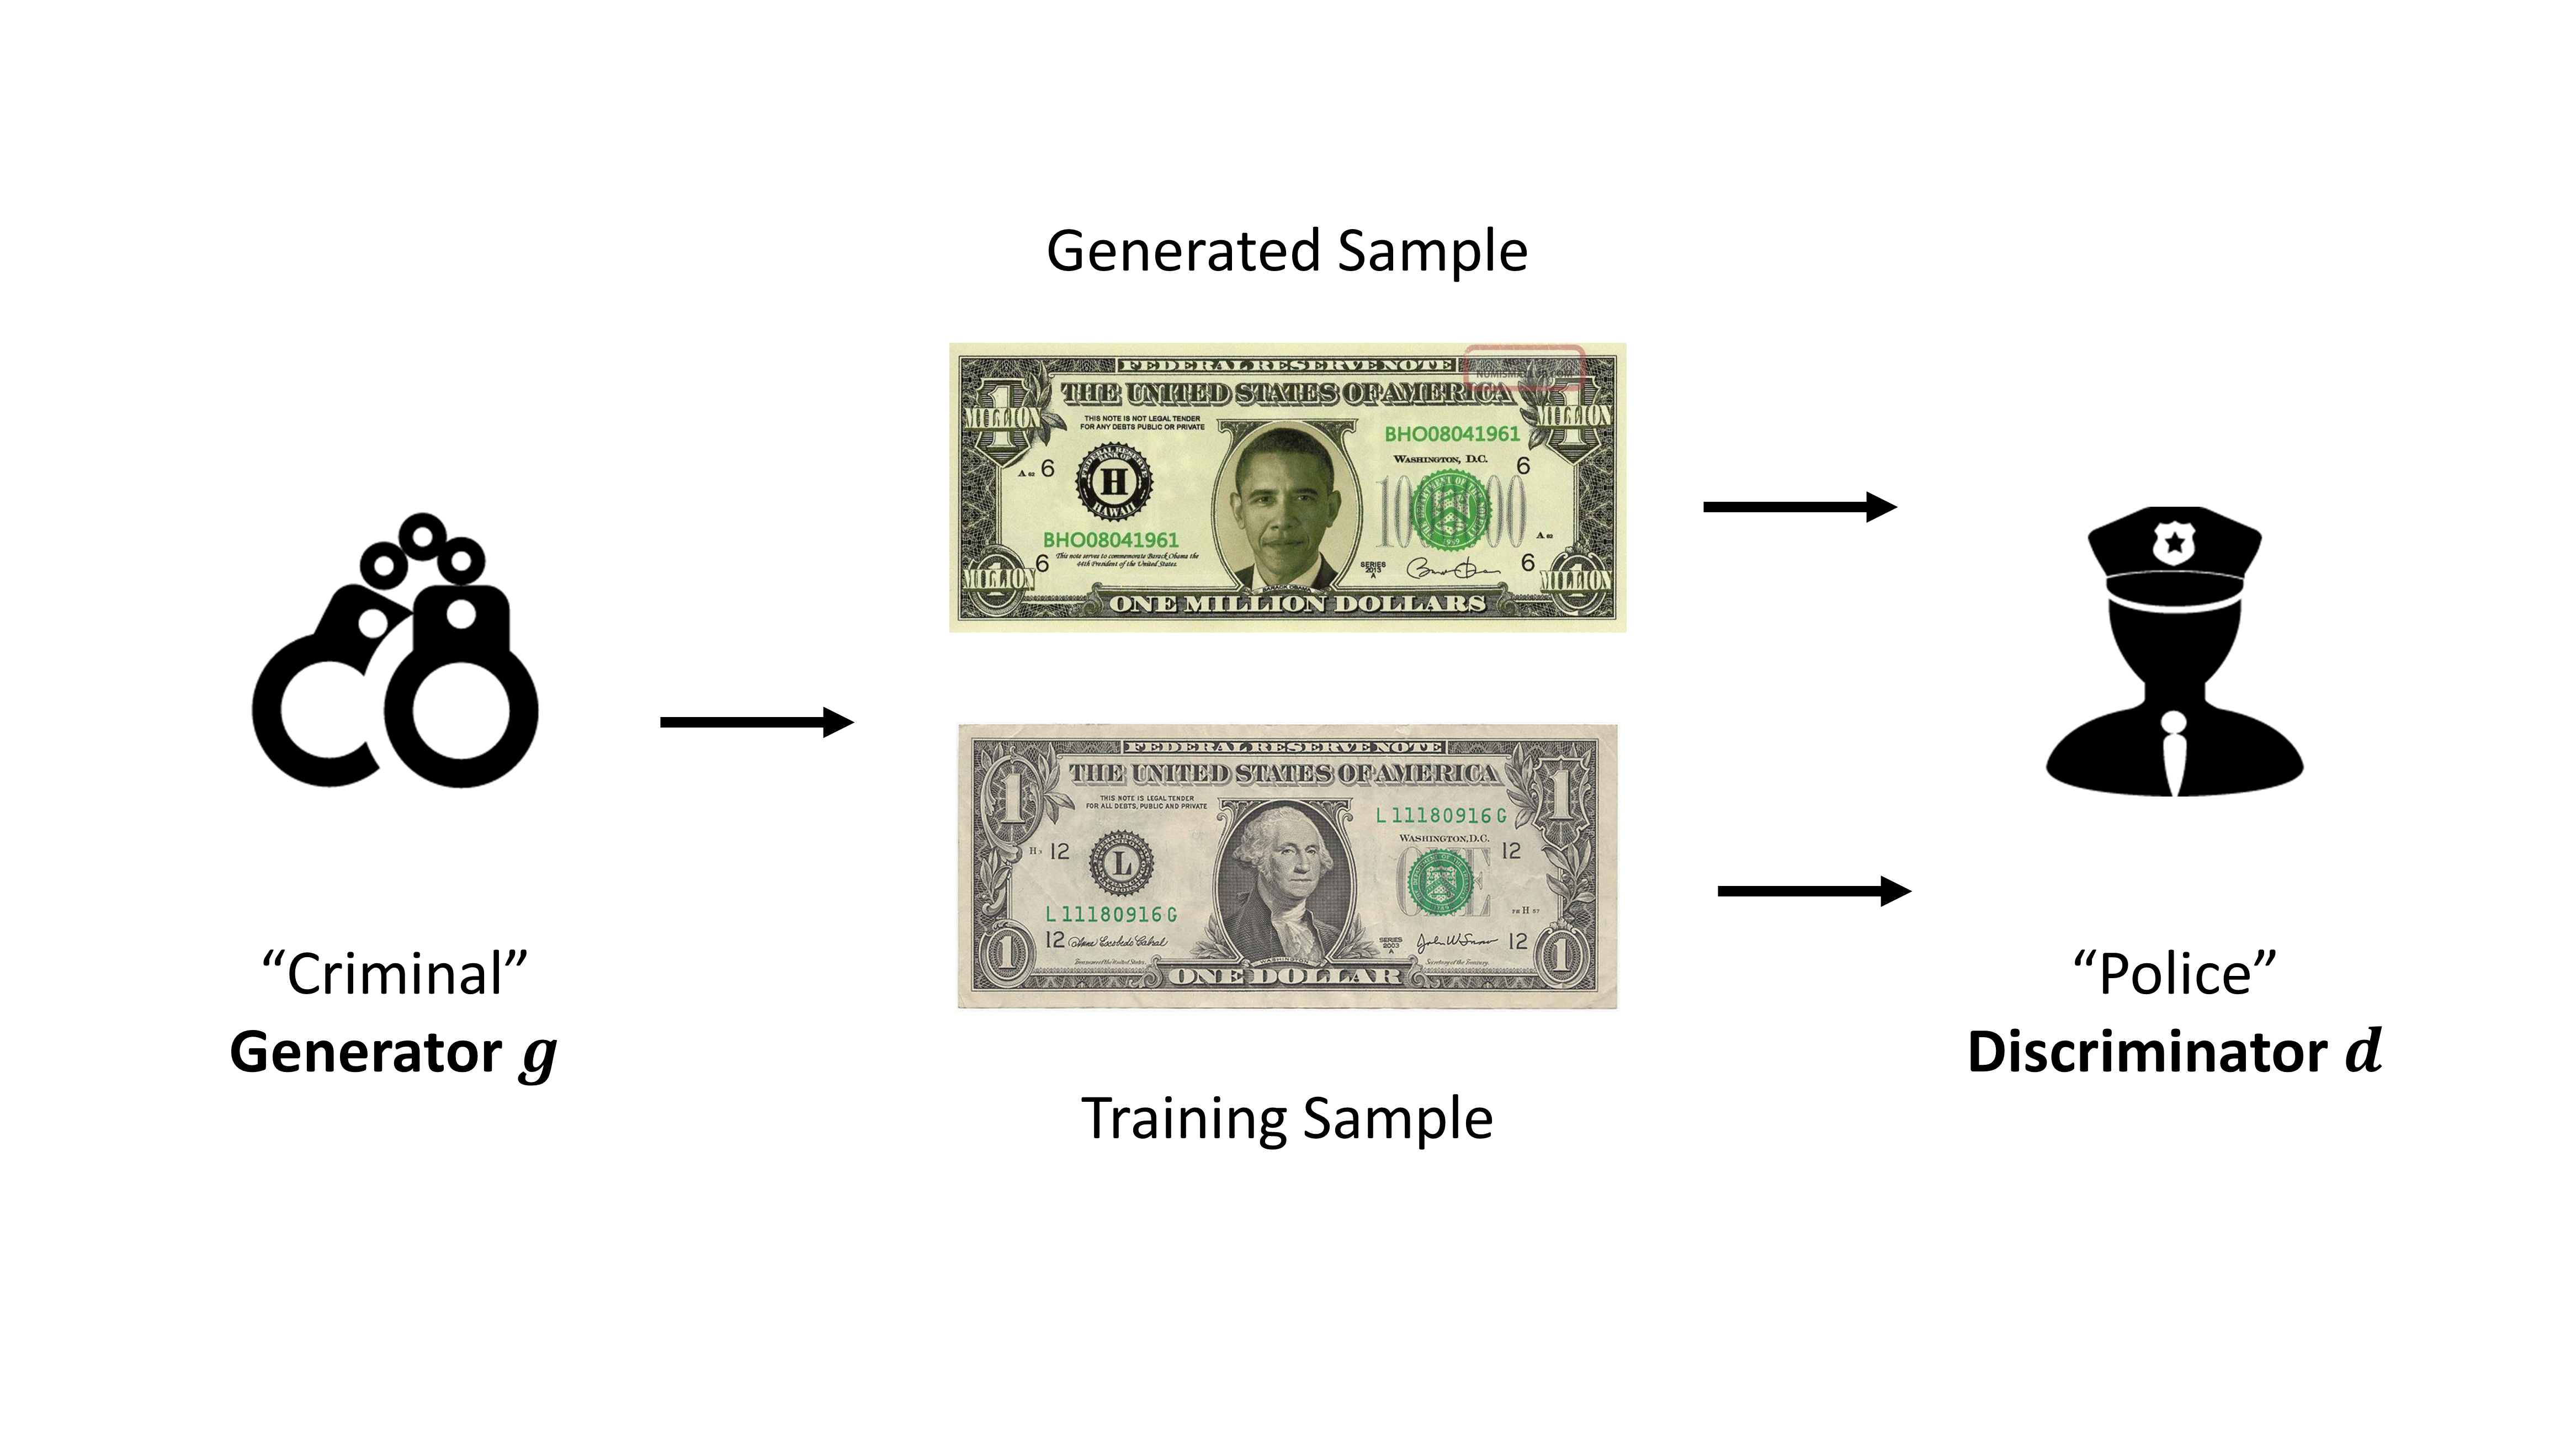
\includegraphics[width=0.9\linewidth]{GAN_conterfeit_cash.png}
	\caption{"Criminal" and "Police" example of GAN model}
	\label{fig:GANcash}
\end{figure}




Underlying scheme of GAN is the competition of generator network and discriminator network in a game theoretic scenario. Intuitively, we can think a scenario of money counterfeiting criminals and policemen. The generator, in this scenario the criminals, want to produce the counterfeited currency without detected by police. And the discriminator, in this case police, want to detect the fake currency. Both criminals and police will improve their methods to compete with each others in the scenario. Ideally,  the competition will reach a zero-sum game, which counterfeits are indistinguishable from the genuine articles, and the discriminator output $ \frac{1}{2} $ everywhere.
 
To formulate the learning of GANs, we can use a function $ v(\bm{\theta}^{(g)}, \bm{\theta}^{(d)}) $. In the contrast, the generator receives $ -v(\bm{\theta}^{(g)} $ as its own payoff. At the convergence $ g^* $, we have:
\[ g^* = \arg \min_{g} \max_{d}v(g, d) \]

And the payoff function $ v $ is given by:
\[ v(\bm{\theta}^{(g)}, \bm{\theta}^{(d)}) = \mathbb{E}_{\mathbf{x}\sim p_{\textit{data}}}\log d(\bm{x})+ \mathbb{E}_{\mathbf{x}\sim p_{\textit{model}}}\log (1- d(\bm{x}))\]

This will drive generator attempt to emulate to the real sample so that it can fool the classifiers. Meantime, the discriminator will attempt to learn to correctly classify real and fake samples.

Original GANs focusing on using convolutional neural network based model to generate image data. By constructing the generator and discriminator using RNNs replacing CNNs, we can build a GANs to generate sequential data. For example, C-RNN-GAN model \cite{mogren2016crnngan} use recurrent neural network based GAN to generate continue music data. 

\begin{figure}[htbp]
	\centering
	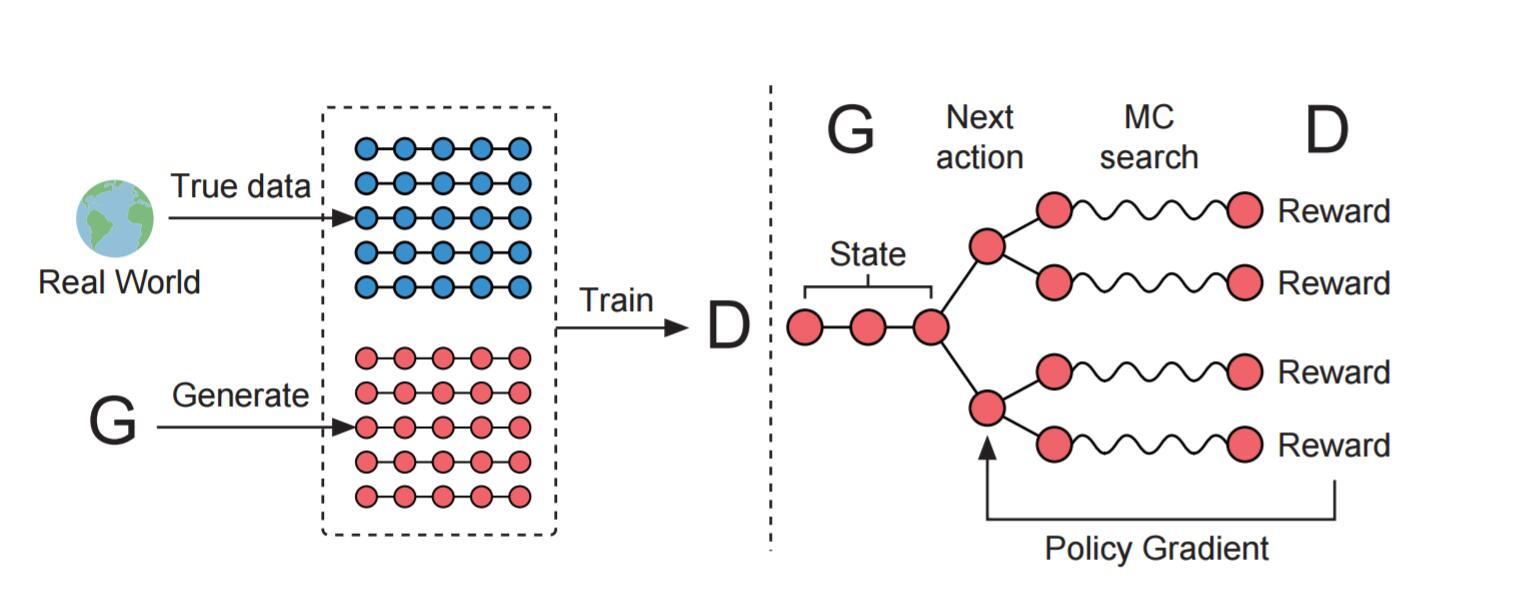
\includegraphics[width=0.9\linewidth]{SwqGAN.jpg}
	\caption{The scheme of SeqGAN model}
	\label{fig:seqGAN}
\end{figure}

However, to apply GANs on sequential data with discrete token is not-trivial \cite{huszar2015}. For discrete sequence, the sampling process cannot be described by a differentiable process we discussed before. So an alternative approach is propose for SeqGAN Model \cite{yu2016seqgan}. The generator in the SeqGAN is treated as an agent of reinforcement learning. Discriminator will evaluate the sequence and the feedback of discriminator will used as guide of learning of generator. The generative model is trained by policy gradient, avoid the challenge of differential of discrete tokens in traditional GANs. SeqGAN model uses RNNs as generator and CNNs for discriminator.